%%%%%%%%%%%%%%%%%%%%%%%%%%%%%%%%%%%%%%%%%%%%%%%
\chapter{Computational Results} \label{chap:comp_method}
%%%%%%%%%%%%%%%%%%%%%%%%%%%%%%%%%%%%%%%%%%%%%%%

In Table \ref{tab:r_over_t}, our vector solutions are computed by
Algorithm \ref{alg:Increasing-Method} for the $\left(\epsilon=1,l=1\right)-\ensuremath{N}_{3,r,4}$
network regarding to $t=2$ and $t=3$. Both construction 1 and 2
provide better results than scalar solutions. 

Construction 1: $\begin{array}{c|c}
\boldsymbol{I}_{t} & \boldsymbol{T}\end{array}$, with $\boldsymbol{T}\in\ensuremath{\mathbb{F}}_{q}^{t\times t\left(h-1\right)}$

Construction 2: $\boldsymbol{T}\in MatrixSpaceUrs\left(t,3t\right)$

Regarding to $t=2$, for a scalar network coding solution we need
a $3-\left(3,1,1\right)_{4}^{c}$ code ($q_{v}=2^{2}=4)$ by Theorem
\ref{theo:scalar_sol_exist}. The largest such code consists of the
21 one-dimensionall subspaces of $\ensuremath{\mathbb{F}}_{4}^{3}$,
each one is contained twice in the code. Therefore, the number of
nodes can be at most 42 for a scalar linear coding solution, while
for vector network coding 89 nodes can be used, i..e. $\mathcal{A}_{q=2}\left(n=6,k=4,t=3;\lambda=2\right)\geq89$
following to Corollary \ref{cor:dual_subspaces}. This is a new lower
bound for $\mathcal{A}_{2}\left(6,4,3;2\right)$ compared to a code
with 51 codewords presented in \cite{Wachter-Zeh:2018}. The smallest
alphabet size for a scalar solution with 89 nodes exists is $q_{s}=8$.
By Equation \ref{eq:r_scalar_max}, there are 73 one-dimensional subspaces
of $\ensuremath{\mathbb{F}}_{8}^{3}$, and each one can be used twice
in the code; therefore, we have in total 146 possible codesword, but
only 89 codewords are required. In this case, the gap size $g=q_{s}-q_{v}=2^{3}-2^{2}=8-4=2^{2},$i.e.
we achieve a gap size $q^{t^{2}/2}$, which is better the asymptotic
behavior in \ref{eq:gap_e1l1h3rs4}.
\begin{defn}[G3]
 Let $\boldsymbol{A},\boldsymbol{B},\boldsymbol{C}\in\ensuremath{\mathbb{F}}_{q}^{n\times m}$.
Then a set $\left\{ \boldsymbol{A},\boldsymbol{B},\boldsymbol{C}\right\} $
forms a subset of $g3$ if

\[
rk\left[\begin{array}{c}
\boldsymbol{A}\\
\boldsymbol{B}\\
\boldsymbol{C}
\end{array}\right]\geq2n
\]

In other words, all $\left\{ \boldsymbol{A},\boldsymbol{B},\boldsymbol{C}\right\} $
span a subspace of $\ensuremath{\mathbb{F}}_{q}^{2n}$ whose dimension
is at least $2n$. We denote $g3_{i}$ as a subset of $g3$:

\[
g3=\left\{ \left\{ \boldsymbol{A},\boldsymbol{B},\boldsymbol{C}\right\} _{i}\right\} =\left\{ g3_{i}\right\} ,i=0,1,2,...,\left|g3\right|-1
\]

with $g3_{i}=\left\{ \boldsymbol{A},\boldsymbol{B},\boldsymbol{C}\right\} _{i}$
\end{defn}
%
\begin{defn}[Relative]
 Let $\boldsymbol{A},\boldsymbol{B},\boldsymbol{C}\in\ensuremath{\mathbb{F}}_{q}^{n\times m}$.
Then $\boldsymbol{C}$ is called a relative of a tuple $\left(\boldsymbol{A},\boldsymbol{B}\right)$
if $\left\{ \boldsymbol{A},\boldsymbol{B},\boldsymbol{C}\right\} \in g3$
and denoted as following:

\[
rel\left[\left(\boldsymbol{A},\boldsymbol{B}\right)\right]=\boldsymbol{C}
\]
\end{defn}
%
\begin{defn}[Sub-relative]
 Let $\boldsymbol{A},\boldsymbol{B},\boldsymbol{C},\boldsymbol{D}\in\ensuremath{\mathbb{F}}_{q}^{n\times m}$.
Then $\boldsymbol{D}$ is called a sub-relative of a tuple $\left(\boldsymbol{A},\boldsymbol{B},\boldsymbol{C}\right)\in g3$
if:

\[
\left\{ \begin{array}{c}
\left\{ \boldsymbol{A},\boldsymbol{B},\boldsymbol{D}\right\} \in g3\\
\left\{ \boldsymbol{A},\boldsymbol{C},\boldsymbol{D}\right\} \in g3\\
\left\{ \boldsymbol{B},\boldsymbol{C},\boldsymbol{D}\right\} \in g3
\end{array}\right.
\]

It is denoted as: 
\[
subrel\left[\left(\boldsymbol{A},\boldsymbol{B},\boldsymbol{C}\right)\right]=\boldsymbol{D}
\]

This definition is reused for a set of 5 or more matrices.
\end{defn}
%
\begin{defn}[MatrixSpace]
 $MatrixSpace(n,m)=\left\{ \boldsymbol{A}:\boldsymbol{A}\in\ensuremath{\mathbb{F}}_{q}^{n\times m}\right\} $
\end{defn}
%
\begin{defn}[MatrixSpace with unique row space]
 $MatrixSpaceUrs(n,m)$ is a subspace of $\ensuremath{\mathbb{F}}_{q}^{n\times m}$,
where any $\boldsymbol{A},\boldsymbol{B}\in\ensuremath{\mathbb{F}}_{q}^{n\times m}$
have their row spaces such that:

\[
\mathcal{R}_{q}\left(\boldsymbol{A}\right)\neq\mathcal{R}_{q}\left(\boldsymbol{B}\right)
\]

where $\mathcal{R}_{q}\left(.\right)$ denotes the row space of a
matrix.
\end{defn}
\begin{algorithm}[H]
\caption{Increasing Method \label{alg:Increasing-Method}}

\textbf{INPUT}: $g3$ of N matrices belonging to $MatrixSpace(n,m)$
or $MatrixSpaceUrs(n,m)$
\begin{enumerate}
\item Create a list of $rel\left[\left(\boldsymbol{A},\boldsymbol{B}\right)\right],\forall\boldsymbol{A},\boldsymbol{B}\in MatrixSpace(n,m),\boldsymbol{A}\neq\boldsymbol{B}$
\item Choose all $\{\boldsymbol{A},\boldsymbol{B}\}$ such that:
\[
\left|rel\left[\left(\boldsymbol{A},\boldsymbol{B}\right)\right]\right|=\left|rel\left[\left(\boldsymbol{A},\boldsymbol{B}\right)\right]\right|_{max}
\]
with an upper bound for the final result set's cardinality $\left|Res\right|\leq UB,UB=\left|rel\left[\left(\boldsymbol{A},\boldsymbol{B}\right)\right]\right|_{max}$.
\item For each found pair set of $\{\boldsymbol{A},\boldsymbol{B}\}$, we
compute the union set of the pair and its Relative, i.e., $\{\boldsymbol{A},\boldsymbol{B}\}\cup rel\left[\left(\boldsymbol{A},\boldsymbol{B}\right)\right]$.
If the union set is repeated or duplicated, we take only the first
pair generating such value. We denote the chosen set as $main\_team\_and\_rel$
\item Considering $main\_team\_and\_rel_{i}\in main\_team\_and\_rel$ with
$i=0,1,2,...,\left|main\_team\_and\_rel\right|-1$, we have 
\[
\begin{array}{c}
rel_{j}\in rel\left[main\_team\_and\_rel_{i}\right]\\
\forall main\_team\_and\_rel_{i}\in main\_team\_and\_rel\\
j=0,1,2,...,\left|main\_team\_and\_rel_{i}\right|-1
\end{array}
\]
to compute $n\_main\_team_{i}$, which is combined by $\{\boldsymbol{A},\boldsymbol{B},rel_{j}\}$
if $\left|subrel\left[\left(\boldsymbol{A},\boldsymbol{B},rel_{j}\right)\right]\right|_{max}$
similarly to step 2.
\item Keep only $n\_main\_team_{i}$ with $\left|subrel\left[\left(n\_main\_team_{i}\right)\right]\right|_{max}$
with $i=0,1,2,...,\left|main\_team\_and\_rel\right|-1$. Similar to
step 3, we also avoid duplicated values here.
\item Repeat step 4, 5, 6 until $\left|subrel\left[\left(n\_main\_team_{i}\right)\right]\right|_{max}=0$
\end{enumerate}
\textbf{OUTPUT}: Get the final result set with all matrices such that:

\[
Res=\left\{ \boldsymbol{X}_{i}:\boldsymbol{X}_{i}\in\ensuremath{\mathbb{F}}_{q}^{n\times m}\right\} ,i=0,1,...,UB
\]

with any 3 combinations of $\left(\boldsymbol{X}_{j},\boldsymbol{X}_{k},\boldsymbol{X}_{t}\right)\in g3,\forall\boldsymbol{X}_{j},\boldsymbol{X}_{k},\boldsymbol{X}_{t}\in Res,\boldsymbol{X}_{j}\neq\boldsymbol{X}_{k}\neq\boldsymbol{X}_{t}$
and $j\neq k\neq t$.
\end{algorithm}

Example 1: Let $n=1,m=2,q=2$. Then we have $N=4$ matrices (vectors):

\[
\begin{array}{c}
\boldsymbol{A}=[0,0]\\
\boldsymbol{B}=[0,1]\\
\boldsymbol{C}=[1,0]\\
\boldsymbol{D}=[1,1]
\end{array}
\]

\uline{Step 1}: Due to, any 3 of them form a matrix with $rk\geq2n$,
we have the relative as following:

\[
\begin{array}{c}
rel\left[\left(\boldsymbol{A},\boldsymbol{B}\right)\right]=[\boldsymbol{C},\boldsymbol{D}]\\
rel\left[\left(\boldsymbol{A},\boldsymbol{C}\right)\right]=[\boldsymbol{B},\boldsymbol{D}]\\
rel\left[\left(\boldsymbol{A},\boldsymbol{D}\right)\right]=[\boldsymbol{B},\boldsymbol{C}]\\
rel\left[\left(\boldsymbol{B},\boldsymbol{C}\right)\right]=[\boldsymbol{A},\boldsymbol{D}]\\
rel\left[\left(\boldsymbol{B},\boldsymbol{D}\right)\right]=[\boldsymbol{A},\boldsymbol{C}]\\
rel\left[\left(\boldsymbol{C},\boldsymbol{D}\right)\right]=[\boldsymbol{A},\boldsymbol{B}]
\end{array}
\]

\uline{Step 2}: We get $UB=2$ and all $\left\{ \boldsymbol{A},\boldsymbol{B}\right\} ,\left\{ \boldsymbol{A},\boldsymbol{C}\right\} ,\left\{ \boldsymbol{A},\boldsymbol{D}\right\} ,\left\{ \boldsymbol{B},\boldsymbol{C}\right\} ,\left\{ \boldsymbol{B},\boldsymbol{D}\right\} ,\left\{ \boldsymbol{C},\boldsymbol{D}\right\} $,
because $\underset{\begin{array}{c}
\forall\boldsymbol{X},\boldsymbol{Y}\in MatrixSpace(1,2)\\
\boldsymbol{X}\neq\boldsymbol{Y}
\end{array}}{max}\left(rel\left[\left(\boldsymbol{X},\boldsymbol{Y}\right)\right]\right)=2$

\uline{Step 3}: Due to $\left\{ \boldsymbol{X},\boldsymbol{Y}\right\} \cup rel\left[\left(\boldsymbol{X},\boldsymbol{Y}\right)\right]=\left\{ \boldsymbol{A},\boldsymbol{B},\boldsymbol{C},\boldsymbol{D}\right\} $
with $\left(\boldsymbol{X},\boldsymbol{Y}\right)$ are all tuples
found in Step 2. We keep only $main\_team\_and\_rel=\left\{ \left(\boldsymbol{A},\boldsymbol{B}\right):rel\left[\left(\boldsymbol{A},\boldsymbol{B}\right)\right]\right\} $

\uline{Step 4}: Regarding to $rel\left[\left(\boldsymbol{A},\boldsymbol{B}\right)\right]$,
we have $rel_{0}=\boldsymbol{C},rel_{1}=\boldsymbol{D}$. Then, $\left|subrel\left[\left(\boldsymbol{A},\boldsymbol{B},rel_{0}\right)\right]\right|=\left|subrel\left[\left(\boldsymbol{A},\boldsymbol{B},rel_{1}\right)\right]\right|=1$,
so we got $n\_main\_team_{0}=\left\{ \boldsymbol{A},\boldsymbol{B},\boldsymbol{C}\right\} $
as the only output of this step.

\uline{Step 5}: Because step 4 gets only $\left\{ \boldsymbol{A},\boldsymbol{B},\boldsymbol{C}\right\} $,
we do not need to proceed anything here.

\uline{Step 6}: We repeat step 4 and 5 once more and we get $Res=\left\{ \boldsymbol{A},\boldsymbol{B},\boldsymbol{C},\boldsymbol{D}\right\} $,
i.e., all the matrices can be used.

~

Example 2: For further understading, we use Figure \ref{fig:rel_example}
for illustration.

In the right, we observe that the size of relative becomes smaller
when its tuple identity is larger, i.e. $\left|rel\left[\left(\boldsymbol{A},\boldsymbol{B}\right)\right]\right|\geq\left|subrel\left[\left(\boldsymbol{A},\boldsymbol{B},\boldsymbol{C}\right)\right]\right|$
or $\left|rel\left[\left(\boldsymbol{A},\boldsymbol{B}\right)\right]\right|\geq\left|subrel\left[\left(\boldsymbol{A},\boldsymbol{B},\boldsymbol{D}\right)\right]\right|$.
It explains why $UB$ is the maximum numbers of matrices that we can
find in $Res$.

Regarding to the left, the visual explanation of $subrel$ is shown.

\begin{figure}[H]
\caption{The vector network coding of $(\epsilon=1,l=1)-\mathcal{N}_{h=3,r,s=4}$
represents as a matrix problem\label{fig:rel_example}}

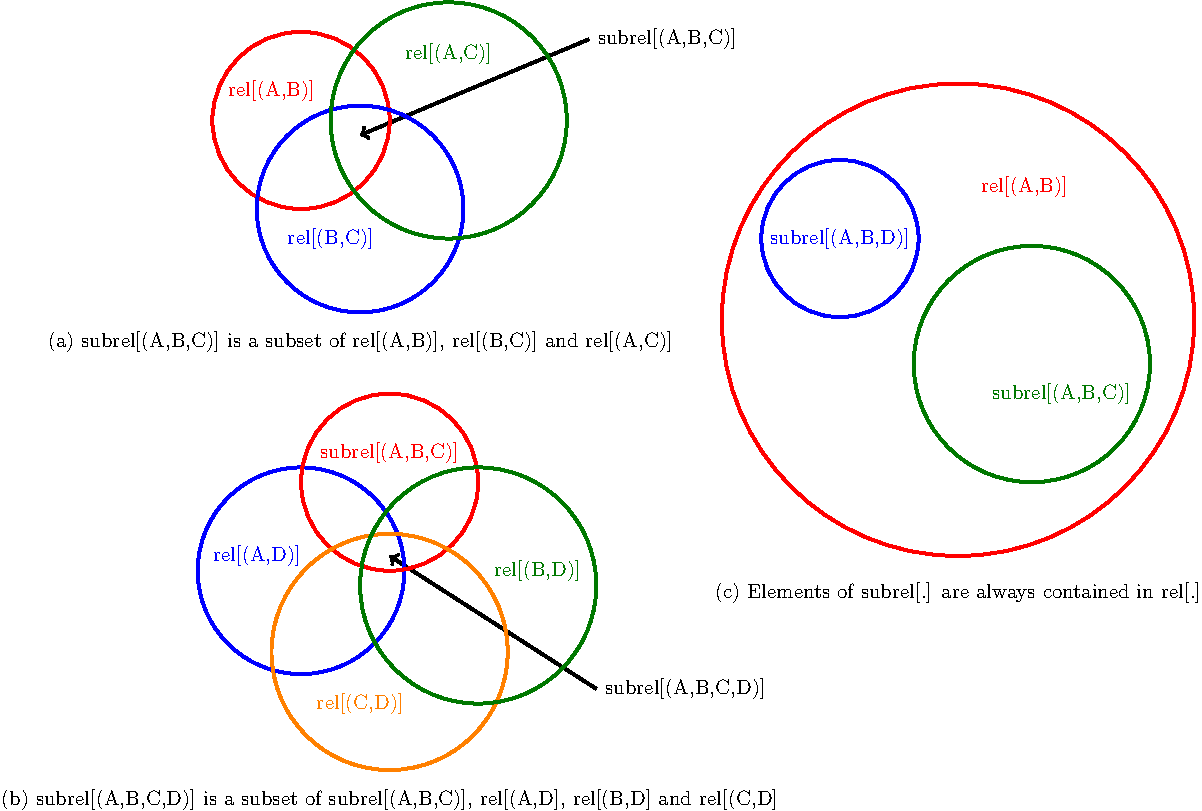
\includegraphics[width=0.5\paperwidth]{E:/Documents/TUM/THESIS/thesisCOD_Ha/figures/rel_example}
\end{figure}

\clearpage